% vim: set ts=4 sw=4 tw=80 noexpandtab:

\documentclass{42-en}

%******************************************************************************%
%                                                                              %
%                                   Prologue                                   %
%                                                                              %
%******************************************************************************%
\usepackage[
    type={CC},
    modifier={by-nc-sa},
    version={4.0},
]{doclicense}
\usepackage{amsmath} % The amsmath package provides commands to typeset matrices with different delimiters. 
\usepackage{epigraph}
\setlength\epigraphwidth{.95\textwidth}
%****************************************************************%
%                  Re/definition of commands                     %
%****************************************************************%

\newcommand{\ailogo}[1]{\def \@ailogo {#1}}\ailogo{assets/42ai_logo.pdf}

%%  Redefine \maketitle
\makeatletter
\def \maketitle {
  \begin{titlepage}
    \begin{center}
	%\begin{figure}[t]
	  %\includegraphics[height=8cm]{\@ailogo}
	  
\includegraphics[height=8cm]{assets/42ai_logo.pdf}
	%\end{figure}
      \vskip 5em
      {\huge \@title}
      \vskip 2em
      {\LARGE \@subtitle}
      \vskip 4em
    \end{center}
    %\begin{center}
	  %\@author
    %\end{center}
	%\vskip 5em
  \vfill
  \begin{center}
    \emph{\summarytitle : \@summary}
  \end{center}
  \vspace{2cm}
  %\vskip 5em
  %\doclicenseThis
  \end{titlepage}
}
\makeatother

\makeatletter
\def \makeheaderfilesforbidden
{
  \noindent
  \begin{tabularx}{\textwidth}{|X X X X|}
    \hline
  \multicolumn{1}{|>{\raggedright}m{1cm}|}
  {\vskip 2mm 
\includegraphics[height=1cm]{assets/42ai_logo.pdf}} &
  \multicolumn{2}{>{\centering}m{12cm}}{\small Exercise : \@exnumber } &
  \multicolumn{1}{ >{\raggedleft}p{1.5cm}|}
%%              {\scriptsize points : \@exscore} \\ \hline
              {} \\ \hline

  \multicolumn{4}{|>{\centering}m{15cm}|}
              {\small \@extitle} \\ \hline

  \multicolumn{4}{|>{\raggedright}m{15cm}|}
              {\small Turn-in directory : \ttfamily
                $ex\@exnumber/$ }
              \\ \hline
  \multicolumn{4}{|>{\raggedright}m{15cm}|}
              {\small Files to turn in : \ttfamily \@exfiles }
              \\ \hline

  \multicolumn{4}{|>{\raggedright}m{15cm}|}
              {\small Forbidden functions : \ttfamily \@exforbidden }
              \\ \hline

%%  \multicolumn{4}{|>{\raggedright}m{15cm}|}
%%              {\small Remarks : \ttfamily \@exnotes }
%%              \\ \hline
\end{tabularx}
%% \exnotes
\exrules
\exmake
\exauthorize{None}
\exforbidden{None}
\extitle{}
\exnumber{}
}
\makeatother

%%  Syntactic highlights
\makeatletter
\newenvironment{pythoncode}{%
  \VerbatimEnvironment
  \usemintedstyle{emacs}
  \minted@resetoptions
  \setkeys{minted@opt}{bgcolor=black,formatcom=\color{lightgrey},fontsize=\scriptsize}
  \begin{figure}[ht!]
    \centering
    \begin{minipage}{16cm}
      \begin{VerbatimOut}{\jobname.pyg}}
{%[
      \end{VerbatimOut}
      \minted@pygmentize{c}
      \DeleteFile{\jobname.pyg}
    \end{minipage}
\end{figure}}
\makeatother

\usemintedstyle{native}

\begin{document}

% =============================================================================%
%                     =====================================                    %

\title{Machine Learning - Module 01}
\subtitle{Univariate Linear Regression}
\author{
  Maxime Choulika (cmaxime), Pierre Peigné (ppeigne), Matthieu David (mdavid)
}

\summary
{
  Today you will implement a method to improve your model's performance: \textbf{gradient descent}.
  Then you will discover the notion of normalization.
}

\maketitle
%******************************************************************************%
%                                                                              %
%                        Section usefull ressources                            %
%                          for ML Modules                                      %
%                                                                              %
%******************************************************************************%


\chapter*{Notions and ressources}

\section*{Notions of the module}
Regularization, overfitting. Regularized loss function, regularized gradient descent.  
Regularized linear regression. Regularized logistic regression.

\section*{Useful Ressources}

You are strongly advise to use the following resource:
\href{https://www.coursera.org/learn/machine-learning}{Machine Learning MOOC - Stanford}
These videos are available at no cost; simply log in, select "Enroll for Free", and choose "audit the course for free" in the popup window.
The following sections of the course are pertinent to today's exercises:

\newpage

\subsection*{Week 3: Classification}

\subsubsection*{Classification with logistic regression (already seen on module 03)}
\begin{itemize}
  \item Motivations
  \item Logistic regression
  \item Decision boundary
\end{itemize}

\subsubsection*{Cost function for logistic regression (already seen on module 03)}
\begin{itemize}
  \item Cost function for logistic regression
  \item Simplified Cost Function for Logistic Regression
\end{itemize}

\subsubsection*{Gradient descent for logistic regression (already seen on module 03)}
\begin{itemize}
  \item Gradient Descent Implementation
\end{itemize}

\subsubsection*{The problem of overfitting (New !!!)}
\begin{itemize}
  \item The problem of overfitting
  \item Addressing overfitting
  \item Cost function with regularization
  \item Regularized linear regression
  \item Regularized logistic regression  
\end{itemize}


\emph{All videos above are available also on this \href{https://youtube.com/playlist?list=PLkDaE6sCZn6FNC6YRfRQc_FbeQrF8BwGI&feature=shared}{Andrew Ng's YouTube playlist}, videos from 31 to 36 (already seen on module 03) and 37 to 41 (new !!!).}
%******************************************************************************%
%                                                                              %
%                        Common Instructions                                   %
%                          for Python Projects                                 %
%                                                                              %
%******************************************************************************%

\chapter*{Common Instructions}
\begin{itemize}
  \item The version of Python recommended to use is 3.7, you can
  check the version of Python with the following command: \texttt{python -V}
  
  \item The norm: during this piscine, it is recommended to follow the
  \href{https://www.python.org/dev/peps/pep-0008/}{PEP 8 standards}, though it is not mandatory.
  You can install \href{https://pypi.org/project/pycodestyle}{pycodestyle} which
  is a tool to check your Python code.
  
  \item The function \texttt{eval} is never allowed.
  
  \item The exercises are ordered from the easiest to the hardest.
  
  \item Your exercises are going to be evaluated by someone else,
  so make sure that your variable names and function names are appropriate and civil. 
  
  \item Your manual is the internet.
  
  \item You can also ask questions on the {https://discord.gg/8Vvb6QMCZq}{42AI} discord.
  
  \item If you find any issue or mistakes in the subject please create an issue on \href{https://github.com/42-AI/bootcamp_python/issues}{42AI repository on Github}.  
  
  \item We encourage you to create test programs for your
  project even though this work \textbf{won't have to be
  submitted and won't be graded}. It will give you a chance
  to easily test your work and your peers’ work. You will find
  those tests especially useful during your defence. Indeed,
  during defence, you are free to use your tests and/or the
  tests of the peer you are evaluating.
  
  \item Submit your work to your assigned git repository. Only the work in the
  git repository will be graded. If Deepthought is assigned to grade your
  work, it will be run after your peer-evaluations.
  If an error happens in any section of your work during Deepthought's grading,
  the evaluation will stop.
\end{itemize}

\newpage
\tableofcontents
\startexercices

%                     =====================================                    %
% =============================================================================%


%******************************************************************************%
%                                                                              %
%                                   Exercises                                  %
%                                                                              %
%******************************************************************************%

% ============================================== %
% ===========================(start ex 00)       %
\chapter{Exercise 00}
%******************************************************************************%
%                                                                              %
%                                 Interlude                                    %
%                         for Machine Learning module                          %
%                                                                              %
%******************************************************************************%

% =============================== %
\section*{Interlude}
% =============================== %
\subsection*{Classification: The Art of Labelling Things}
% ******************************* %
Over the last three modules you have implemented your first machine learning algorithm.\\
\\
You are now familiar the three-steps cycle we follow when we build \textbf{learning algorithms}:
\\
\begin{figure}[!h]
    \centering
    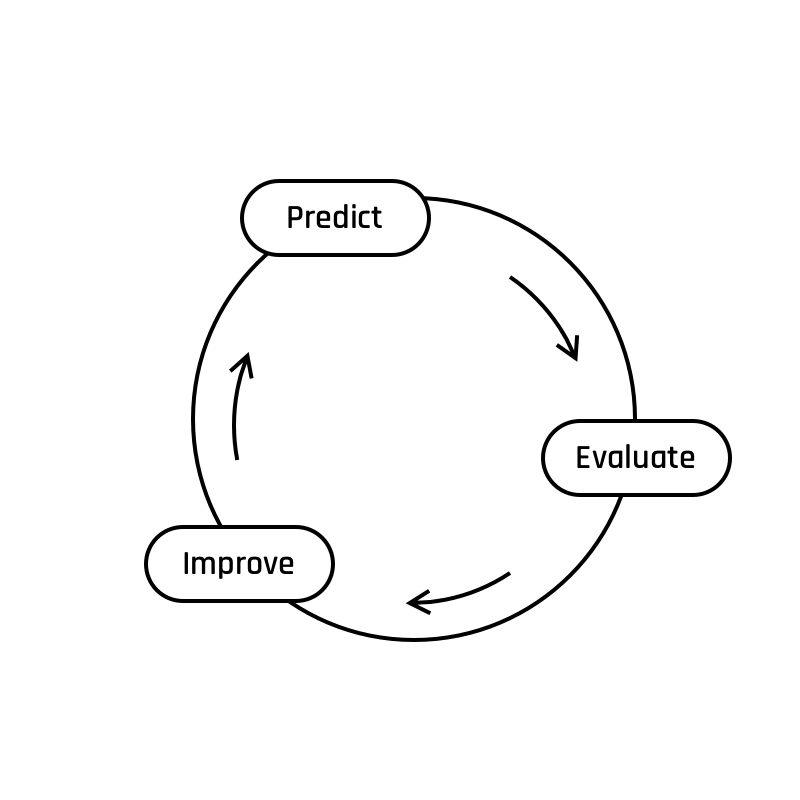
\includegraphics[scale=0.25]{assets/Default.png}
    %\caption{The Learning Cycle}
\end{figure}
\\
The first algorithm you discovered, \textbf{Multivariate Linear Regression}, can now be used to predict a numerical value, based on several features.
This algorithm uses gradient descent to optimize its loss function.\\
\\
Now let's introduce your first \textbf{classification algorithm}: the notorious \textbf{Logistic Regression.}
\hint{regression vs classification; discrete vs continuous values}
\newpage
\noindent{\textbf{Logistic regression} performs a \textit{classification task}, which means that you are not predicting a numerical value (like price, age, grades...) 
but \textbf{categories}, or \textbf{labels} (like dog, cat, sick/healty...)}.
\\
\warn{
    Don't be confused by the word \textit{'regression'} in \textbf{Logistic Regression}.
    It really is a \textit{classification task}! The name is a bit tricky but you will quickly get used to it.
    Once again: \textbf{Logistic Regression is a classification algorithm} which assigns a label/category/class to a given example.
}
\info{
    In this module we will use the following terms interchangeably: \textbf{class}, \textbf{category}, and \textbf{label}.
    They all refer to the \textit{groups} to which each training example can be assigned to, in a classification task.
}

% =============================== %
\subsection*{Predict I: Introducing the Sigmoid Function}
% ******************************* %

\begin{figure}[!h]
    \centering
    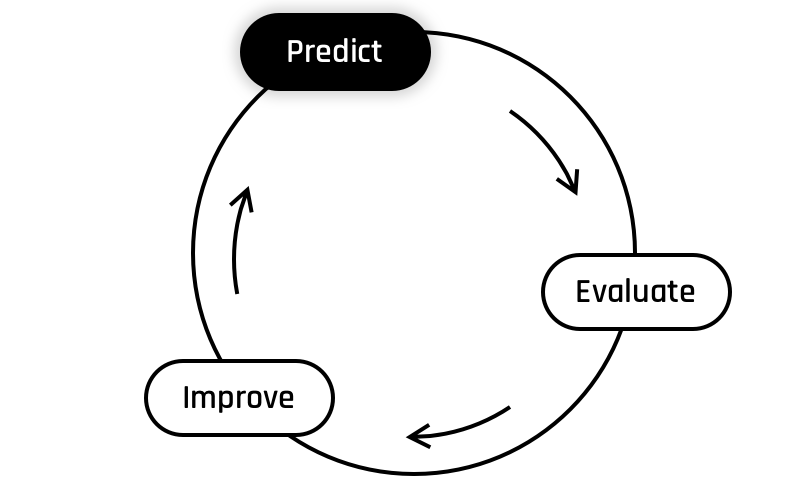
\includegraphics[scale=0.25]{assets/Predict.png}
    %\caption{The Learning Cycle - Predict}
\end{figure}

% =============================== %
\subsubsection*{Formulating a Hypothesis}
% ******************************* %
Remember that a hypothesis, denoted $h(\theta)$, is an equation that combines a set of \textbf{features} (that characterizes an example) with \textbf{parameters} in order to output a \textbf{prediction}.\\
\\
Remember the hypothesis we used in linear regression?\\
$$
h(\theta) = \theta_0 + \theta_{1} x_{1}^{(i)} + \dots + \theta_{n} x_{n}^{(i)} = \theta \cdot x'^{(i)}
$$
\newline
It worked fine to predict continuous values, but could we also use it to tell, for example, 
if a patient is sick or not?
That's a yes-or-no question, so the output from the hypothesis function should reflect that.\\
\\
To get started, we will assign each class a numerical value: sick patients will be 
assigned a value of 1, and healthy patients will be assigned a value of 0.\\
The goal will be to build a hypothesis that outputs a probability that a patient is sick as a float number in the range of [0, 1].\\
\\
The good news is that we can keep the linear equation we already worked with!\\
\\
All we need to do is squash its output through another function that is bounded between 0 and 1.\\
\\
That's the purpose of the \textbf{Sigmoid function} and your next assignment is to implement it!

\newpage
\extitle{Linear Gradient - Iterative Version}
\turnindir{ex00}
\exnumber{00}
\exfiles{gradient.py}
\exforbidden{None}
\makeheaderfilesforbidden

% ================================== %
\section*{Objective}
% ---------------------------------- %
Understand and manipulate the notion of gradient and gradient descent in machine learning.\
You must write a function that computes the \textbf{\textit{gradient}} of the loss function.
It must compute a partial derivative with respect to each theta parameter separately, and return the vector gradient.
The partial derivatives can be calculated with the following formulas:  
$$
\nabla(J)_0 = \frac{1}{m}\sum_{i=1}^{m}(h_{\theta}(x^{(i)}) - y^{(i)})
$$

$$
\nabla(J)_1 = \frac{1}{m}\sum_{i=1}^{m}(h_{\theta}(x^{(i)}) - y^{(i)})x^{(i)}
$$

Where:
\begin{itemize}
  \item $\nabla(J)$ is the gradient vector of size $2 \times 1$, (this strange symbol : $\nabla$ is called nabla)
  \item $x$ is a vector of dimension $m$,
  \item $y$ is a vector of dimension $m$,
  \item $x^{(i)}$ is the i$^\text{th}$ component of vector $x$,
  \item $y^{(i)}$ is the i$^\text{th}$ component of vector $y$,
  \item $\nabla(J)_j$ is the j$^\text{th}$ component of $\nabla(J)$,
  \item $h_{\theta}(x^{(i)})$ corresponds to the model's prediction of $y^{(i)}$.
\end{itemize}

% ================================== %
\section*{Hypothesis Notation}
% ---------------------------------- %
$h_{\theta}(x^{(i)})$ is the same as what we previously noted $\hat{y}^{(i)}$.  
The two notations are equivalent.
They represent the model's prediction (or estimation) of the ${y}^{(i)}$ value.
If you follow Andrew Ng's course material on Coursera, you will see him using the former notation.

As a reminder:
$h_{\theta}(x^{(i)}) = \theta_0 + \theta_1x^{(i)}$


% ================================== %
\section*{Instructions}
% ---------------------------------- %

In the \texttt{gradient.py} file create the following function as per the instructions given below:

\begin{minted}[bgcolor=darcula-back,formatcom=\color{lightgrey},fontsize=\scriptsize]{python}
  def simple_gradient(x, y, theta):
    """Computes a gradient vector from three non-empty numpy.array, without any for-loop.
       The three arrays must have compatible shapes.
    Args:
      x: has to be an numpy.array, a vector of shape m * 1.
      y: has to be an numpy.array, a vector of shape m * 1.
      theta: has to be an numpy.array, a 2 * 1 vector.
    Return:
      The gradient as a numpy.array, a vector of shape 2 * 1.
      None if x, y, or theta are empty numpy.array.
      None if x, y and theta do not have compatible shapes.
      None if x, y or theta is not of the expected type.
    Raises:
      This function should not raise any Exception.
    """
    ... Your code ...
\end{minted}

% ================================== %
\section*{Examples}
% ---------------------------------- %

\begin{minted}[bgcolor=darcula-back,formatcom=\color{lightgrey},fontsize=\scriptsize]{python}
import numpy as np
x = np.array([12.4956442, 21.5007972, 31.5527382, 48.9145838, 57.5088733]).reshape((-1, 1))
y = np.array([37.4013816, 36.1473236, 45.7655287, 46.6793434, 59.5585554]).reshape((-1, 1))

# Example 0:
theta1 = np.array([2, 0.7]).reshape((-1, 1))
simple_gradient(x, y, theta1)
# Output:
array([[-19.0342574], [-586.66875564]])

# Example 1:
theta2 = np.array([1, -0.4]).reshape((-1, 1))
simple_gradient(x, y, theta2)
# Output:
array([[-57.86823748], [-2230.12297889]])
\end{minted}

% ===========================(fin ex 00)         %
% ============================================== %

\newpage

% ============================================== %
% ===========================(start ex 01)       %
\chapter{Exercise 01}
%******************************************************************************%
%                                                                              %
%                                 Interlude                                    %
%                         for Machine Learning module                          %
%                                                                              %
%******************************************************************************%

% =============================== %
\section*{Linear Algebra Tricks part II}
% ******************************* %

If you tried to run your code on a very large dataset, you would find that it sometimes takes a (very) long time to execute!
That's because it doesn't use the power of Python libraries that are optimized for matrix operations.\\
\newline
Remember the linear algebra trick from the previous module? Let's use it again!  
If you concatenate a column of $1$'s to the left of the $x$ vector, you get what we called matrix $X'$.   
$$
X' = \begin{bmatrix} 1 & x^{(1)} \\ \vdots & \vdots \\ 1 & x^{(m)}\end{bmatrix}
$$
This transformation is very convenient because we can rewrite each $1$ as $x_0^{(i)}$, and each $x^{(i)}$ as $x_1^{(i)}$.
So now the $X'$ matrix looks like this:
$$
X' = \begin{bmatrix} x_0^{(1)} & x_1^{(1)} \\ \vdots & \vdots \\ x_0^{(m)} & x_1^{(m)}\end{bmatrix}
$$
Notice that each $x^{(i)}$ example becomes a vector made of $(x^{(i)}_0, x^{(i)}_1)$.  
The $0$ and $1$ indices on the $x$ features correspond to the indices of the $\theta$ parameters with which they will be multiplied.\\
\newline
Why does this matter?
Well, if we take the equation from the previous exercise:

$$
\nabla(J)_0 = \frac{1}{m}\sum_{i=1}^{m}(h_{\theta}(x^{(i)}) - y^{(i)})
$$
We can multiply it by $1$ without changing its value:
$$
\nabla(J)_0 = \frac{1}{m}\sum_{i=1}^{m}(h_{\theta}(x^{(i)}) - y^{(i)}) \cdot 1
$$
And rewrite $1$ as $x_0^{(i)}$:
$$
\nabla(J)_0 = \frac{1}{m}\sum_{i=1}^{m}(h_{\theta}(x^{(i)}) - y^{(i)})x_{0}^{(i)}
$$
This means that the equation for $\nabla(J)_0$ is now similar to the equation we had for $\nabla(J)_1$, so they can both be captured by ONE \textbf{generic equation}:
$$
\begin{matrix}
\nabla(J)_j = \frac{1}{m}\sum_{i=1}^{m}(h_{\theta}(x^{(i)}) - y^{(i)})x_{j}^{(i)} & & \text{ for j = 0, 1}    
\end{matrix}
$$
And as you probably suspected, a generic equation opens the door to vectorization...

% =============================== %
\subsection*{Vectorizing the Gradient Calculation}
% ******************************* %
Now it's time to learn how to calculate the entire gradient in one short, pretty, linear algebra equation!  
\begin{itemize}
    \item First, we'll use the $X'$ matrix and our vectorized hypothesis equation $h_{\theta}(x)=X'\theta$
    $$
    \begin{matrix}
    \nabla(J)_j = \frac{1}{m} (X'\theta - y)X'_{j} & & \text{ for j = 0, 1}
    \end{matrix}
    $$
    
    \item Second, we need to tweak the equation a bit so that it directly returns a $\nabla(J)$ vector containing both $\nabla(J)_0$ and $\nabla(J)_1$.
    
    $$
    \nabla(J) = \frac{1}{m} {X'}^T(X'\theta - y)    
    $$
\end{itemize}
If the equation does not seems obvious, play a bit with your vectors, on paper and in your code, until you get it.\\

% =============================== %
\subsubsection*{Notation Remark}
% ******************************* %
${X'}^T$: You might wonder what the $^T$ is for.
It means the $X'$ matrix must be \textbf{transposed}.\\
\newline
Transposing a matrix flips it on its diagonal so that its rows become its columns and \textit{vice-versa}.
Here we need to make sure that matrix dimensions are appropriate and allow for multiplication, and to multiply the right items together.
\newpage
\extitle{Linear Gradient - Vectorized Version}
\turnindir{ex01}
\exnumber{01}
\exfiles{vec\_gradient.py}
\exforbidden{None}
\makeheaderfilesforbidden

% ================================= %
\section*{Objective}
% --------------------------------- %
Understand and manipulate the notion of gradient and gradient descent in machine learning.\
You must implement the following formula as a function:

$$
\nabla(J) = \frac{1}{m} {X'}^T(X'\theta - y)
$$  

Where:
\begin{itemize}
  \item $\nabla(J)$ is a vector of dimension $2 \times 1$.
  \item $X'$ is a \textbf{matrix} of dimensions $(m \times 2)$,
  \item ${X'}^T$ is the transpose of $X'$. Its dimensions are $(2 \times m)$,
  \item $y$ is a vector of dimension $m$,
  \item $\theta$ is a vector of dimension $2 \times 1$. 
\end{itemize}
  
Be careful:
\begin{itemize}
  \item the $x$ you will get as an input is an $m$ vector,
  \item $\theta$ is a $2 \times 1$ vector. You have to transform $x$ to fit the dimension of $\theta$!
\end{itemize}

% ================================= %
\section*{Instructions}
% --------------------------------- %
In the \texttt{vec\_gradient.py} file create the following function as per the instructions given below:
\par
\begin{minted}[bgcolor=darcula-back,formatcom=\color{lightgrey},fontsize=\scriptsize]{python}
def gradient(x, y, theta):
    """Computes a gradient vector from three non-empty numpy.array, without any for loop.
       The three arrays must have compatible shapes.
    Args:
      x: has to be a numpy.array, a matrix of shape m * 1.
      y: has to be a numpy.array, a vector of shape m * 1.
      theta: has to be a numpy.array, a 2 * 1 vector.
    Return:
      The gradient as a numpy.ndarray, a vector of dimension 2 * 1.
      None if x, y, or theta is an empty numpy.ndarray.
      None if x, y and theta do not have compatible dimensions.
    Raises:
      This function should not raise any Exception.
    """
    ... Your code ...
\end{minted}

% ================================= %
\section*{Examples}
% --------------------------------- %

\begin{minted}[bgcolor=darcula-back,formatcom=\color{lightgrey},fontsize=\scriptsize]{python}
import numpy as np
x = np.array([12.4956442, 21.5007972, 31.5527382, 48.9145838, 57.5088733]).reshape((-1, 1))
y = np.array([37.4013816, 36.1473236, 45.7655287, 46.6793434, 59.5585554]).reshape((-1, 1))

# Example 0:
theta1 = np.array([2, 0.7]).reshape((-1, 1))
gradient(x, y, theta1)
# Output:
array([[-19.0342574], [-586.66875564]])

# Example 1:
theta2 = np.array([1, -0.4]).reshape((-1, 1))
gradient(x, y, theta2)
# Output:
array([[-57.86823748], [-2230.12297889]])
\end{minted}

% ===========================(fin ex 01)         %
% ============================================== %

\newpage

% ============================================== %
% ===========================(start ex 02)       %
\chapter{Exercise 02}
%******************************************************************************%
%                                                                              %
%                                 Interlude                                    %
%                         for Machine Learning module                          %
%                                                                              %
%******************************************************************************%

\section*{Interlude - Predict, Evaluate, Improve}

\epigraph
{A computer program is said to learn from experience E, with respect to some
class of tasks T, and performance measure P, if its performance at tasks in T,
as measured by P, improves with experience E.}{\textit{Tom Mitchell,\\Machine Learning, 1997}}

\begin{quote}{}

\end{quote}

In other words to learn you have to improve.\\
To improve you have to evaluate your performance.\\
To evaluate your performance you need to start performing on the task you want to be good at.


One of the most common tasks in Machine Learning is \textbf{prediction}.\\  
This will be your algorithm's task.\\
This will be your task.  

\begin{figure}[h!]
  \centering
  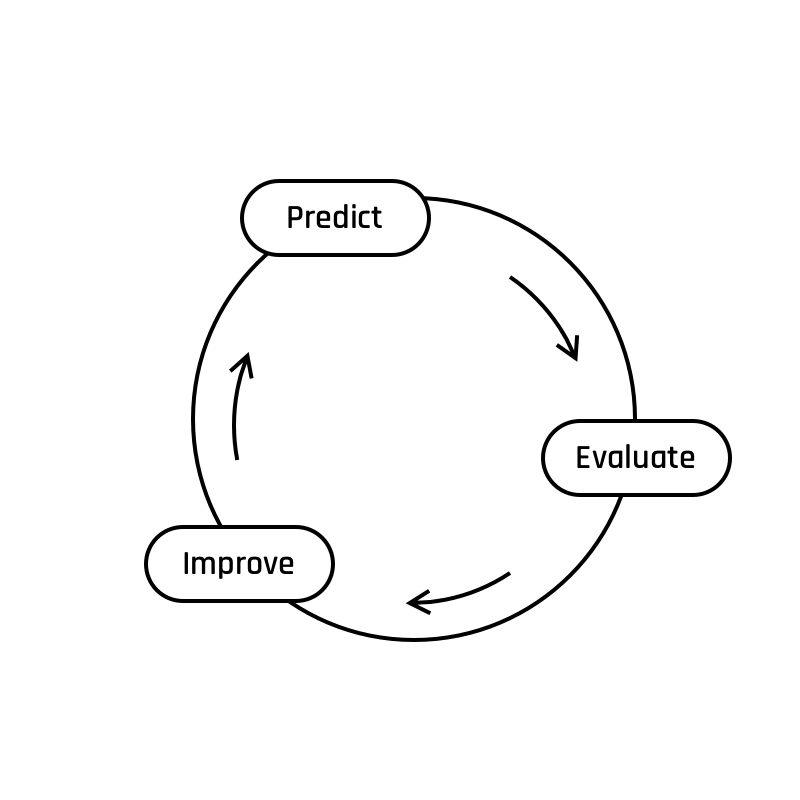
\includegraphics[scale=0.25]{assets/Default.png}
  \caption{cycle neutral}
\end{figure}

\section*{Predict}

\begin{figure}[h!]
  \centering
  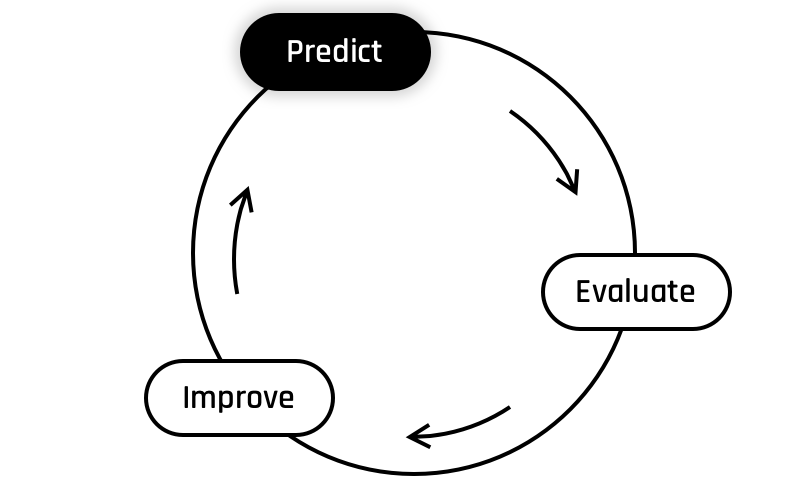
\includegraphics[scale=0.25]{assets/Predict.png}
  \caption{cycle predict}
\end{figure}

\subsection*{A very simple model}

We have some data. We want to model it.  
\begin{itemize}
    \item First we need to \textit{make an assumption}, or hypothesis, \textit{about the structure of the data and the relationship between the variables}.  
    \item Then we can \textit{apply that hypothesis to our data to make predictions}.
\end{itemize}

$$
hypothesis(data) = predictions
$$

\subsubsection*{Hypothesis}
Let's start with a very simple and intuitive \textbf{hypothesis} on how the price of a spaceship can be predicted based on the power of its engines.\\
We will consider that \textit{the more powerful the engines are, the more expensive the spaceship is}.\\
Furthermore, we will assume that the price increase is \textbf{proportional} to the power increase. In other words, we will look for a \textbf{linear relationship} between the two variables.

This means that we will formulate the price prediction with a \textbf{linear equation}, that you might be already familiar with:

$$
\hat{y} = ax + b
$$

We add the \texttt{\^} symbol over the $y$ to specify that $\hat{y}$ \textit{(pronounced y-hat)} is a \textbf{prediction} (or estimation) of the real value of $y$. The prediction is calculated with the \textbf{parameters} $a$ and $b$ and the input value $x$.

For example, if $a = 5$ and $b = 33$, then $\hat{y} = 5x + 33$.

But in Machine Learning, we don't like using the letters $a$ and $b$. Instead we will use the following notation:

$$
\hat{y} = \theta_0 + \theta_1 x
$$

So if $\theta_0 = 33$ and $\theta_1 = 5$, then $\hat{y} = 33+ 5x$.

To recap, this linear equation is our \textbf{hypothesis}. Then, all we will need to do is find the right values for our parameters $\theta_0$ and $\theta_1$ and we will get a fully-functional prediction \textbf{model}.


\subsubsection*{Predictions}
Now, how can we generate a set of predictions on an entire dataset? Let's consider a dataset containing $m$ data points (or space ships), called \textbf{examples}.

What we do is stack the $x$ and $\hat{y}$ values of all examples in vectors of length $m$. The relation between the elements in our vectors can then be represented with the following formula:

$$
\begin{matrix}
\hat{y}^{(i)} = \theta_0 + \theta_1 x^{(i)} & & \text{ for i = 1, ..., m}
\end{matrix}
$$  

Where:
\begin{itemize}
    \item $\hat{y}^{(i)}$ is the $i^{th}$ component of vector $y$
    \item $x^{(i)}$ is the $i^{th}$ component of vector $x$   
\end{itemize}

Which can be experessed as:

$$
\hat{y} = \begin{bmatrix}\theta_0 + \theta_1 \times x^{(1)} \\ \vdots \\  \theta_0 + \theta_1 \times x^{(m)}\ \end{bmatrix}
$$  

For example,

$$
\text{given } \theta = \begin{bmatrix}33 \\ 5 \end{bmatrix} \text{ and } x = \begin{bmatrix}1 \\ 3 \end{bmatrix} \text{: }
$$

$$
\hat{y} = h_{\theta}(x) = \begin{bmatrix} 33 +  5 \times 1 \\ 33 + 5 \times 3\end{bmatrix}  = \begin{bmatrix} 38 \\ 48 \end{bmatrix} 
$$

\newpage

\subsection*{More information}

\subsubsection*{Why the $\theta$ notation?}

You might have two questions at the moment:
\begin{itemize}
    \item \textbf{WTF is that weird  symbol?}
    This strange symbol, $\theta$, is called "theta".
    
    \item \textbf{Why use this notation instead of $a$ and $b$, like we're used to?}
    Despite its seeming more complicated at first, the theta notation is actually meant to simplify your equations later on. Why?
    $a$ and $b$ are good for a model with two parameters, but you will soon need to build more complex models that take into account more variables than just $x$.
    You could add more letters like this:  $\hat{y} = ax_1 + bx_2 + cx_3 + ... + yx_{25} + z$  
    But how do you go beyond 26 parameters? And how easily can you tell what parameter is associated with, let's say, $x_{19}$? That's why it becomes more handy to describe all your parameters using the theta notation and indices.
    With $\theta$, you just have to increment the number to name the parameter:
    $\hat{y} = \theta_0 + \theta_1 x_1 + \theta_2 x_2 + ... + \theta_{2468} x_{2468}$ ... Easy right?
\end{itemize}


\subsubsection*{Another common notation}

$$
\begin{matrix} & & \hat{y} & = & h_{\theta}(x)\end{matrix}
$$

Because $\hat{y}$ is calculated with our linear hypothesis using $\theta$ and $x$, it is sometimes written as $h_{\theta}(x)$.
The $h$ stands for \textit{hypothesis}, and can be read as \textit{"the result of our hypothesis h given x and theta"}.

Then if $x = 7$, we can calculate:
$\hat{y} = h_{\theta}(x) = 33 + 5 \times 7 = 68$
We can now say that according to our linear model, the \textbf{predicted value} of $y$ given ($x = 7$) is 68.

\newpage
\extitle{Gradient Descent}
\turnindir{ex02}
\exnumber{02}
\exfiles{fit.py}
\exforbidden{any function that calculates derivatives for you}
\makeheaderfilesforbidden

% ================================= %
\section*{Objective}
% --------------------------------- %
Understand and manipulate the notion of gradient and gradient descent in machine learning.\
Be able to explain what it means to \textbf{\textit{fit}} a Machine Learning model to a dataset.\
Implement a function that performs \textbf{Linear Gradient Descent} (LGD).


% ================================= %
\section*{Instructions}
% --------------------------------- %
In this exercise, you will implement linear gradient descent to fit your model to the dataset.

The pseudocode for the algorithm is the following:

$$
\begin{matrix}
&\text{repeat until convergence:} & \{ \\
&	\text{compute } \nabla{(J)}  \\
&	\theta_0 := \theta_0 - \alpha \nabla(J)_0  \\
&	\theta_1 := \theta_1 - \alpha \nabla(J)_1\\
	\}
\end{matrix}
$$

Where:
\begin{itemize}
  \item $\alpha$ (alpha) is the \textit{learning rate}. It's a small float number (usually between 0 and 1),
  \item For now, "reapeat until convergence" will mean to simply repeat for max\_iter (a number that you will choose wisely).
\end{itemize}

You are expected to write a function named \texttt{fit\_} as per the instructions below:

\begin{minted}[bgcolor=darcula-back,formatcom=\color{lightgrey},fontsize=\scriptsize]{python}
def fit_(x, y, theta, alpha, max_iter):
	"""
	Description:
		Fits the model to the training dataset contained in x and y.
	Args:
		x: has to be a numpy.ndarray, a vector of dimension m * 1: (number of training examples, 1).
		y: has to be a numpy.ndarray, a vector of dimension m * 1: (number of training examples, 1).
		theta: has to be a numpy.ndarray, a vector of dimension 2 * 1.
		alpha: has to be a float, the learning rate
		max_iter: has to be an int, the number of iterations done during the gradient descent
	Returns:
		new_theta: numpy.ndarray, a vector of dimension 2 * 1.
		None if there is a matching dimension problem.
	Raises:
		This function should not raise any Exception.
	"""
		... your code here ...
\end{minted}

Hopefully, you have already written a function to calculate the linear gradient.


% ================================= %
\section*{Examples}
% --------------------------------- %
\begin{minted}[bgcolor=darcula-back,formatcom=\color{lightgrey},fontsize=\scriptsize]{python}
import numpy as np
x = np.array([[12.4956442], [21.5007972], [31.5527382], [48.9145838], [57.5088733]])
y = np.array([[37.4013816], [36.1473236], [45.7655287], [46.6793434], [59.5585554]])
theta= np.array([1, 1]).reshape((-1, 1))

# Example 0:
theta1 = fit_(x, y, theta, alpha=5e-8, max_iter=1500000)
theta1
# Output:
array([[1.40709365],
		[1.1150909 ]])

# Example 1:
predict(x, theta1)
# Output:
array([[15.3408728 ],
		[25.38243697],
		[36.59126492],
		[55.95130097],
		[65.53471499]])
\end{minted}

\info{
\begin{itemize}
  \item You can create more training data by generating an $x$ array with random values and computing the corresponding $y$ vector as a linear expression of $x$. You can then fit a model on this artificial data and find out if it comes out with the same $\theta$ coefficients that first you used.
  \item It is possible that $\theta_0$ and $\theta_1$ become "nan". In that case, it means you probably used a learning rate that is too large.
\end{itemize}
}
% ===========================(fin ex 02)         %
% ============================================== %

\newpage

% ============================================== %
% ===========================(start ex 03)       %
\chapter{Exercise 03}
\extitle{Linear Regression with Class}
\turnindir{ex03}
\exnumber{03}
\exfiles{my\_linear\_regression.py}
\exforbidden{any functions from sklearn}
\makeheaderfilesforbidden

% ================================= %
\section*{Objective}
% --------------------------------- %
Write a class that contains all methods necessary to perform linear regression.


% ================================= %
\section*{Instructions}
% --------------------------------- %
In this exercise, you will not learn anything new but don't worry, it's for your own good.
You are expected to write your own \texttt{MyLinearRegression} class which looks similar to the class available in Scikit-learn:
\texttt{sklearn.linear\_model.LinearRegression}
\par
\begin{minted}[bgcolor=darcula-back,formatcom=\color{lightgrey},fontsize=\scriptsize]{python}
class MyLinearRegression():
	"""
	Description:
		My personnal linear regression class to fit like a boss.
	"""
	def __init__(self,  thetas, alpha=0.001, max_iter=1000):
				self.alpha = alpha
				self.max_iter = max_iter
				self.thetas = thetas

	#... other methods ...
\end{minted}
\newpage
You will add the following methods:
\begin{itemize}
  \item \texttt{fit\_(self, x, y)},
  \item \texttt{predict\_(self, x)},
  \item \texttt{cost\_elem\_(self, y, y\_hat)},
  \item \texttt{cost\_(self, y, y\_hat)}.
\end{itemize}

You have already implemented these functions,
you just need a few adjustments so that they all work well within your \texttt{MyLinearRegression} class.


% ================================= %
\section*{Examples}
% --------------------------------- %
\begin{minted}[bgcolor=darcula-back,formatcom=\color{lightgrey},fontsize=\scriptsize]{python}
import numpy as np
from mylinearregression import MyLinearRegression as MyLR
x = np.array([[12.4956442], [21.5007972], [31.5527382], [48.9145838], [57.5088733]])
y = np.array([[37.4013816], [36.1473236], [45.7655287], [46.6793434], [59.5585554]])

lr1 = MyLR([2, 0.7])

# Example 0.0:
lr1.predict_(x)
# Output:
array([[10.74695094],
		[17.05055804],
		[24.08691674],
		[36.24020866],
		[42.25621131]])

# Example 0.1:
MyLR.cost_elem_(y, lr1.predict(x))
# Output:
array([[710.45867381],
		[364.68645485],
		[469.96221651],
		[108.97553412],
		[299.37111101]])

# Example 0.2:
MyLR.cost_(y, lr1.predict(x))
# Output:
195.34539903032385

# Example 1.0:
lr2 = MyLR([1, 1], 5e-8, 1500000)
lr2.fit_(x, y)
lr2.thetas
# Output:
array([[1.40709365],
		[1.1150909 ]])

# Example 1.1:
lr2.predict_(x)
# Output:
array([[15.3408728 ],
		[25.38243697],
		[36.59126492],
		[55.95130097],
		[65.53471499]])

# Example 1.2:
MyLR.cost_elem_(y, lr2.predict(x))
# Output:
array([[486.66604863],
		[115.88278416],
		[ 84.16711596],
		[ 85.96919719],
		[ 35.71448348]])

# Example 1.3:
MyLR.cost_(y, lr2.predict(x))
# Output:
80.83996294128525
\end{minted}

% ===========================(fin ex 03)         %
% ============================================== %

\newpage

% ============================================== %
% ===========================(start ex 04)       %
\chapter{Exercise 04}
\extitle{Practicing Linear Regression}
\turnindir{ex04}
\exnumber{04}
\exfiles{linear\_model.py, are\_blue\_pills\_magics.csv}
\exforbidden{sklearn}
\makeheaderfilesforbidden


% ================================= %
\section*{Objective}
% --------------------------------- %
Evaluate a linear regression model on a very small dataset, with a given hypothesis function $h$.\
Manipulate the loss function $J$, plot it, and briefly analyze the plot.

% ================================= %
\section*{Instructions}
% --------------------------------- %
You can find in the \texttt{resources} folder a tiny dataset called \texttt{are\_blue\_pills\_magics.csv} which gives you the driving performance of space pilots as a function of the quantity of the "blue pills" they took before the test.
You have a description of the data in the file named \texttt{are\_blue\_pills\_magics.txt}.
As your hypothesis function $h$, you will choose:

$$
h_{\theta}(x) = \theta_0 + \theta_1x
$$

Where $x$ is the variable, and $\theta_0$ and $\theta_1$ are the coefficients of the hypothesis.
The hypothesis is a function of $x$.

\textbf{You are strongly encouraged to use the class you have implement in the previous exercise}.
\newline

Your program must:
\begin{itemize}
  \item Read the dataset from the csv file,
  \item perform a linear regression, 
\end{itemize}
\newpage
Then you will model the data and plot 2 different graphs:
\begin{itemize}
  \item A graph with the data and the hypothesis you get for the spacecraft piloting score versus the quantity of "blue pills" (see figure \ref{best fit for score vs micrograms})
  \begin{figure}[!h]
    \centering
    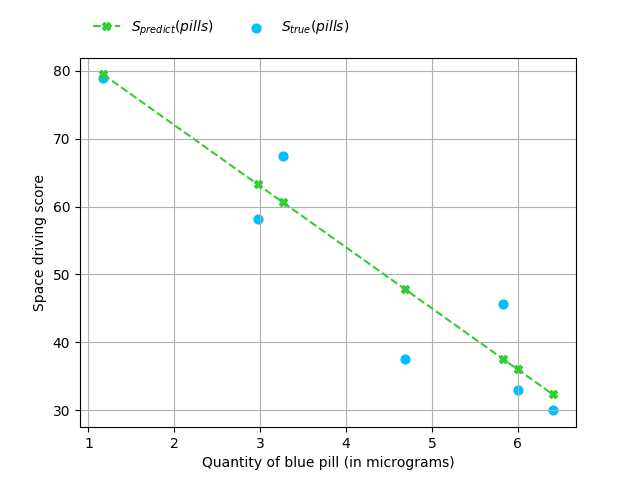
\includegraphics[scale=0.6]{assets/ex04_score_vs_bluepills.png}
    \caption{Space driving score as a function of the quantity of blue pill (in micrograms). In blue the real values and in green the predicted values.}
    \label{best fit for score vs micrograms}
  \end{figure}
  
  \item The cost function $J(\theta)$ in function of the $\theta$ values (see figure \ref{loss function qs function of theta1 and theta0}),
  \begin{figure}[!h]
    \centering
    \includegraphics[scale=0.6]{assets/ex04_J_vs_t1.png}
    \caption{Evolution of the loss function $J$ as a function of $\theta_1$ for different values of $\theta_0$.}
    \label{loss function qs function of theta1 and theta0}
  \end{figure}
   
  \item You will calculate the MSE of the hypothesis you chose (you know how to do it already).
\end{itemize}

% ================================= %
\section*{Examples}
% ================================= %
\begin{minted}[bgcolor=darcula-back,formatcom=\color{lightgrey},fontsize=\scriptsize]{python}
import pandas as pd
import numpy as np
from sklearn.metrics import mean_squared_error
from mylinearregression import MyLinearRegression as MyLR

data = pd.read_csv("are_blue_pills_magic.csv")
Xpill = np.array(data[Micrograms]).reshape(-1,1)
Yscore = np.array(data[Score]).reshape(-1,1)

linear_model1 = MyLR(np.array([[89.0], [-8]]))
linear_model2 = MyLR(np.array([[89.0], [-6]]))
Y_model1 = linear_model1.predict_(Xpill)
Y_model2 = linear_model2.predict_(Xpill)

print(MyLR.mse_(Yscore, Y_model1))
# 57.60304285714282
print(mean_squared_error(Yscore, Y_model1))
# 57.603042857142825
print(MyLR.mse_(Yscore, Y_model2))
# 232.16344285714285
print(mean_squared_error(Yscore, Y_model2))
# 232.16344285714285
\end{minted}
\par
Here, the use of scikit learn is to ensure that our code is performing as expected. The use of scikit learn is forbidden in the code you will turn-in.

\hint{
There is no method named \texttt{.mse\_} in sklearn's LinearRegression class, but there is also a method named \texttt{.score}.
The \texttt{.score} method corresponds to the $R^2$ score.
The metric MSE is available in the \texttt{sklearn.metrics} module.
}
% ===========================(fin ex 04)         %
% ============================================== %

\newpage

% ============================================== %
% ===========================(start ex 05)       %
\chapter{Exercise 05}
%******************************************************************************%
%                                                                              %
%                                 Interlude                                    %
%                         for Machine Learning module                          %
%                                                                              %
%******************************************************************************%

\section*{Interlude - Normalization}

The values inside the $x$ vector can vary quite a lot in magnitude,
depending on the type of data you are working with.
For example, if your dataset contains distances between planets in km, the numbers will be huge.
On the other hand, if you are working with planet masses expressed as a fraction of the solar system's total mass, the numbers will be very small (between 0 and 1).
Both cases may slow down convergence in Gradient Descent (or even sometimes prevent convergence at all).
To avoid that kind of situation, normalization is a very effective way to proceed.


The idea behind this technique is straightforward: \textbf{scaling the data}.  


With normalization, you can transform your $x$ vector into a new $x'$ vector whose values range between $[-1, 1]$ more or less. Doing this allows you to see much more easily how a training example compares to the other ones:
\begin{itemize}
    \item If an $x'$ value is close to $1$, you know it's among the largest in the dataset
    \item If an $x'$ value is close to $0$, you know it's close to the median
    \item If an $x'$ value is close to $-1$, you know it's among the smallest
\end{itemize}

So with the upcoming normalization techniques, you'll be able to map your data to two different value ranges: $[0, 1]$ or $[-1, 1]$. Your algorithm will like it and thank you for it.  

\newpage
\extitle{Normalization I: Z-score Standardization}
\turnindir{ex05}
\exnumber{05}
\exfiles{z-score.py}
\exforbidden{None}
\makeheaderfilesforbidden



% ================================= %
\section*{Objective}
% --------------------------------- %
Introduction to standardization/normalization methods.\
You must implement the following formula as a function:
$$
\begin{matrix}
 x'^{(i)} = \frac{x^{(i)} - \frac{1}{m} \sum_{i = 1}^{m} x^{(i)}}{\sqrt{\frac{1}{m - 1} \sum_{i = 1}^{m} (x^{(i)} - \frac{1}{m} \sum_{i = 1}^{m} x^{(i)})^{2}}} & &\text{ for $i$ in $1, ..., m$} 
\end{matrix}
$$

Where:
\begin{itemize}
  \item $x$ is a vector of dimension $m$,
  \item $x^{(i)}$ is the i$^\text{th}$ component of the $x$ vector,
  \item $x'$ is the normalized version of the $x$ vector.
\end{itemize}

The equation is much easier to understand in the following form:

$$
\begin{matrix}
x'^{(i)} = \frac{x^{(i)} - \mu}{\sigma} & &\text{ for $i$ in $1, ..., m$}
\end{matrix}
$$

This should remind you something from \textbf{TinyStatistician}...

Nope?

Ok let's do a quick recap:
\begin{itemize}
  \item $\mu$ is the mean of $x$,
  \item $\sigma$ is the standard deviation of $x$.
\end{itemize}

% ================================= %
\section*{Instructions}
% --------------------------------- %
In the \texttt{zscore.py} file, write the \texttt{zscore} function as per the instructions given below:

\begin{minted}[bgcolor=darcula-back,formatcom=\color{lightgrey},fontsize=\scriptsize]{python}
def zscore(x):
	"""Computes the normalized version of a non-empty numpy.ndarray using the z-score standardization.
	Args:
		x: has to be an numpy.ndarray, a vector.
	Returns:
		x' as a numpy.ndarray. 
		None if x is a non-empty numpy.ndarray or not a numpy.ndarray.
	Raises:
		This function shouldn't raise any Exception.
	"""
	... Your code ...
\end{minted}


% ================================= %
\section*{Examples}
% --------------------------------- %
\begin{minted}[bgcolor=darcula-back,formatcom=\color{lightgrey},fontsize=\scriptsize]{python}
# Example 1:
X = numpy.array([0, 15, -9, 7, 12, 3, -21])
zscore(X)
# Output:
array([-0.08620324,  1.2068453 , -0.86203236,  0.51721942,  0.94823559,
		0.17240647, -1.89647119])

# Example 2:
Y = np.array([2, 14, -13, 5, 12, 4, -19]).reshape((-1, 1))
zscore(Y)
# Output:
array([ 0.11267619,  1.16432067, -1.20187941,  0.37558731,  0.98904659,
		0.28795027, -1.72770165])
\end{minted}


% ===========================(fin ex 05)         %
% ============================================== %

\newpage

% ============================================== %
% ===========================(start ex 06)       %
\chapter{Exercise 06}
\extitle{Normalization II: Min-max Standardization}
\turnindir{ex06}
\exnumber{06}
\exfiles{minmax.py}
\exforbidden{None}
\makeheaderfilesforbidden


% ================================= %
\section*{Objective}
% --------------------------------- %
Introduction to standardization/normalization methods.\
Implement another normalization method.

You must implement the following formula as a function: 

$$
\begin{matrix}
  x'^{(i)} = \frac{x^{(i)} - min(x)}{max(x) - min(x)} & & \text{ for $i = 1, ..., m$}
\end{matrix}
$$

Where:
\begin{itemize}
  \item $x$ is a vector of dimension $m$,
  \item $x^{(i)}$ is the i$^\text{th}$ component of vector $x$,
  \item $min(x)$ is the minimum value found among the components of vector $x$,
  \item $max(x)$ is the maximum value found among the components of vector $x$.
\end{itemize}

You will notice that this min-max standardization doesn't scale the values to the $[-1,1]$ range.
What do you think the final range will be?

% ================================= %
\section*{Instructions}
% --------------------------------- %
In the \texttt{minmax.py} file, create the \texttt{minmax} function as per the instructions given below:

\begin{minted}[bgcolor=darcula-back,formatcom=\color{lightgrey},fontsize=\scriptsize]{python}
def minmax(x):
    """Computes the normalized version of a non-empty numpy.array using the min-max standardization.
    Args:
        x: has to be an numpy.array, a vector.
    Return:
        x' as a numpy.array. 
        None if x is a non-empty numpy.array or not a numpy.array.
        None if x is not of the expected type.
    Raises:
        This function shouldn't raise any Exception.
    """
    ... Your code ...
\end{minted}

% ================================= %
\section*{Examples}
% --------------------------------- %
\begin{minted}[bgcolor=darcula-back,formatcom=\color{lightgrey},fontsize=\scriptsize]{python}
# Example 1:
X = np.array([[0],[ 15],[ -9],[ 7],[ 12],[ 3],[ -21]])
minmax(X)
# Output:
array([0.58333333, 1., 0.33333333, 0.77777778, 0.91666667,
       0.66666667, 0.])


# Example 2:
Y = np.array([[2],[ 14],[ -13],[ 5],[ 12],[ 4],[ -19]])
minmax(Y)
# Output:
array([0.63636364, 1., 0.18181818, 0.72727273, 0.93939394,
       0.6969697 , 0.])
\end{minted}

% ===========================(fin ex 06)         %
% ============================================== %

\newpage

% ============================================== %
% ===========================(start ex 07)       %
\chapter{Conclusion - What you have learned}

The excercises serie is finished, well done!
Based on all the knowledges tackled today, you should be able to discuss and answer the following questions:

\begin{enumerate}
  \item What is a hypothesis and what is its goal?  
  \item What is the loss function and what does it represent?   
  \item What is Linear Gradient Descent and what does it do?  
  (hint: you have to talk about J, its gradient and the theta parameters...)  
  \item What happens if you choose a learning rate that is too large?
  \item What happens if you choose a very small learning rate, but still a sufficient number of cycles?
  \item Can you explain MSE and what it measures?
\end{enumerate}


% ===========================(fin ex 07)         %
% ============================================== %

\newpage

% ================================= %
\section*{Contact}
% --------------------------------- %
You can contact 42AI association by email: contact@42ai.fr\\
You can join the association on \href{https://join.slack.com/t/42-ai/shared_invite/zt-ebccw5r7-YPkDM6xOiYRPjqJXkrKgcA}{42AI slack}
and/or posutale to \href{https://forms.gle/VAFuREWaLmaqZw2D8}{one of the association teams}.

% ================================= %
\section*{Acknowledgements}
% --------------------------------- %
The modules Python \& ML is the result of a collective work, we would like to thanks:
\begin{itemize}
  \item Maxime Choulika (cmaxime),
  \item Pierre Peigné (ppeigne),
  \item Matthieu David (mdavid).
\end{itemize}
who supervised the creation, the enhancement and this present transcription.

\begin{itemize}
  \item Amric Trudel (amric@42ai.fr)
  \item Benjamin Carlier (bcarlier@student.42.fr)
  \item Pablo Clement (pclement@student.42.fr)
\end{itemize}
for your investment for the creation and development of these modules.

\begin{itemize}
  \item Richard Blanc (riblanc@student.42.fr)
  \item Solveig Gaydon Ohl (sgaydon-@student.42.fr)
  \item Quentin Feuillade Montixi (qfeuilla@student.42.fr)
\end{itemize}
who betatest the first version of the modules of Machine Learning.
\vfill
\doclicenseThis

\end{document}
